\documentclass{mp}

\graphicspath{{04_warunkowe/bayes/},{04_warunkowe/}}

\makeatletter
\newlength{\koza@len}
\newcommand{\koza}[2][]
{
\setlength{\koza@len}{1357pt*\real{#2}}

\begingroup\edef\x
{
	\endgroup
	\noexpand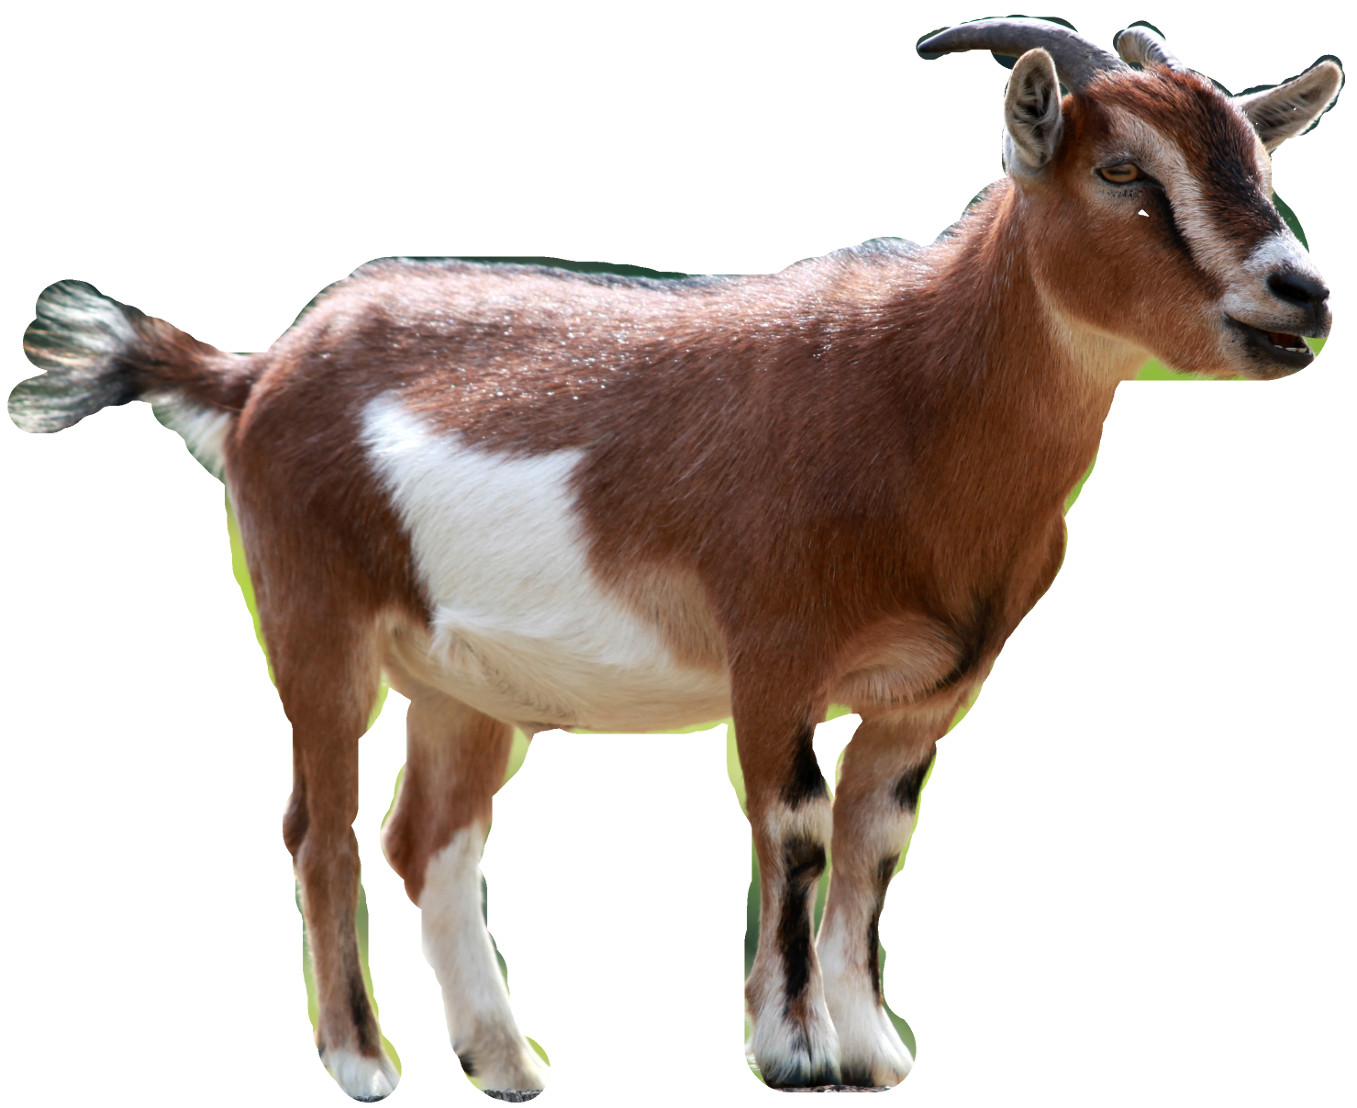
\includegraphics[clip, #1, viewport=0 0 {\the\koza@len} 1108pt]{monty_hall/koza.jpg}
	\noexpand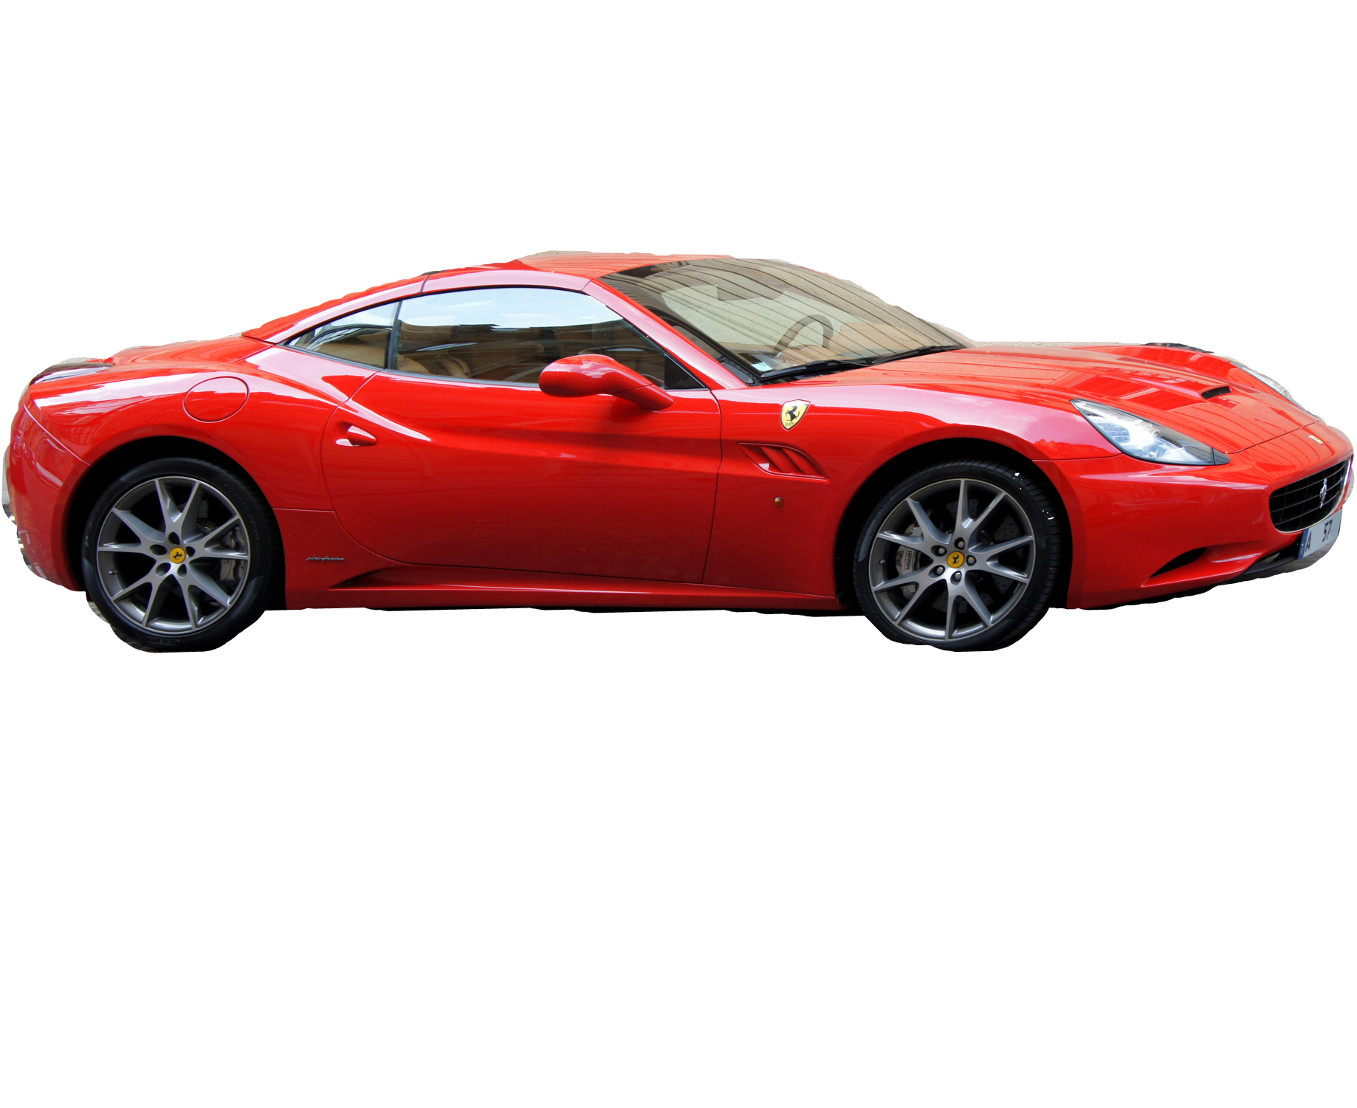
\includegraphics[clip, #1, viewport={\the\koza@len} 0 1357pt 1108pt]{monty_hall/ferrari.jpg}
}
\x
}
\makeatother


\subtitle{Prawdopodobieństwo warunkowe}
\begin{document}
\frame{\titlepage}
\part{Podstawy interpretacji wyników badań medycznych}
\frame{\partpage}
\begin{frame}{Badanie raka}
\newcommand{\eR}{\ensuremath\textcolor{color2}{R}}
\newcommand{\enR}{\ensuremath\textcolor{color3}{R'}}
\newcommand{\eM}{\ensuremath\textcolor{color4}{M}}
\only<1-7>{
\begin{block}{}
Grupa kobiet w wieku 40 lat bierze udział w przesiewowej mammografi, znane są następujące fakty:
\begin{itemize}
\item $\only<3->{P(\eR)=}1\%$ ma raka \only<2>{($\eR$)}
\item $\only<3->{P(\eM|\eR)=}80\%$ kobiet chorych na raka \only<2>{($\eR$) }otrzymuje pozytywny wyniki mammografi \only<2>{($\eM$)}
\item $\only<3->{P(\eM|\enR)=}9{,}6\%$ kobiet zdrowych \only<2>{($\enR$) }otrzymuje pozytywny wynik mammografii \only<2>{($\eM$)}
\end{itemize}
Pewna kobieta otrzymała pozytywny wyniki mammografi. Jakie jest prawdopodobieństwo\only<4->{ $P(\eR|\eM)$}, że ma raka?
\end{block}
}
\begin{tikzpicture}[x=0.1cm,y=.5cm]
\only<5->
{
\fill [color2] (0,0) rectangle (1,1);
\fill [color3] (1,0) rectangle (100, 1);
\draw (0,0) rectangle (100,1);
\node at (50,1.5) {$100\%$};
\node [color2] at ($(2.5,-0.5)$) {$1\%$};
\node [color3] at ($(1,-0.5)+.5*(99,0)$) {$99\%$};
}
\only<6->
{
\draw [dashed] (0,0) -- (0,-2);
\draw [dashed] (1,0) -- (45,-2);
\fill [color4] (0,-2) rectangle ++($(0,-1)+.8*(45,0)$);
\draw [color2] (0,-2) rectangle ++(45,-1);
\node [color2] at ($(0,-1.5)+.5*(45,0)$) {$100\%$};
\node [color4] at ($(0,-3.5)+.5*.8*(45,0)$) {$80\%$};
}
\only<7->
{
\draw [dashed] (1,0) -- (55,-2);
\draw [dashed] (100,0) -- (100,-2);
\fill [color4] (55,-2) rectangle ++($(0,-1)+.096*(45,0)$);
\draw [color3] (55,-2) rectangle ++(45,-1);
\node [color3] at ($(55,-1.5)+.5*(45,0)$) {$100\%$};
\node [color4] at ($(55,-3.5)+.7*.096*(45,0)$) {$9{,}6\%$};
}
\end{tikzpicture}
\only<1>{\footnotesize Źródło: \url{http://www.yudkowsky.net/rational/bayes}}
\let\eR\undefined
\let\enR\undefined
\let\eM\undefined
\note<7>{
	\begin{gather*}
		P(M)=P(M|R)P(R)+P(M|R')P(R')=\frac{8}{10}\frac{1}{100}+\frac{96}{1000}\frac{99}{100}=\frac{10304}{100000} \\
		P(R|M)=\frac{P(R\cap M)}{P(M)}=\frac{P(M|R)P(R)}{P(M)}=\frac{8}{10}\frac{1}{100}\frac{100000}{10304}=\frac{800}{10304}\approx 7{,}76\%
	\end{gather*}
}
\end{frame}
\part{Formalizm matematyczny}
\frame{\partpage}
\begin{frame}{Prawdopodobieństwo warunkowe}
\[ P(A|B)=\frac{P(A\cap B)}{P(B)} \qquad P(B)>0 \]
\only<2>
{
\begin{block}{Twierdzenie o prawdopodobieństwie warunkowym}
Prawdopodobieństwo warunkowe spełnia aksjomaty Kołmogorowa
\end{block}
}
\only<3>
{
	\begin{block}{Twierdzenie}
	\begin{align*}
		P(A_1 \cap A_2)= & P(A_2|A_1)P(A_1) \\
		P(A_1 \cap A_2 \cap A_3)=& P(A_3|A_1\cap A_2)P(A_2|A_1)P(A_1) \\
		P(A_1 \cap A_2 \cap A_3\cap A_4)=& P(A_4|A_1\cap A_2\cap A_3) P(A_3|A_1\cap A_2)P(A_2|A_1)P(A_1) \\
		\ldots
	\end{align*}
	\end{block}
}
\only<4-5>
{
\begin{block}{\only<4>{Twierdzenie o prawdopodobieństwie całkowitym (zupełnym)}\only<5>{Twierdzenie Bayesa}}
Niech:
\begin{itemize}
\item $A_1, A_2, \ldots \in \mathcal{A}$
\item $\forall i\neq j\colon A_i\cap A_j\equiv \emptyset$
\item $A_1\cup A_2\cup \ldots \equiv \Omega$
\item $\forall i\colon P(A_i)>0$
\end{itemize}
wtedy:
\[
\only<4>{P(B)=P(B|A_1)P(A_1)+P(B|A_2)P(A_2)+\ldots}
\only<5>{P(A_i|B)=\frac{P(B|A_i)P(A_i)}{P(B|A_1)P(A_1)+P(B|A_2)P(A_2)+\ldots}}
\]
\end{block}
}
\end{frame}
\begin{frame}{Thomas Bayes}
\begin{center}
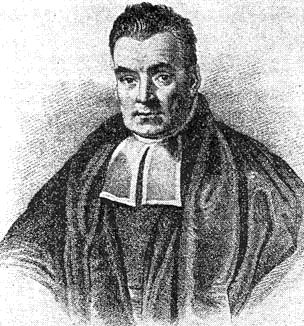
\includegraphics[height=.7\textheight]{Thomas_Bayes.png}\\
Thomas Bayes (1702--1761)
\end{center}
{\tiny \url{http://commons.wikimedia.org/wiki/File:Thomas_Bayes.gif} domena publiczna}
\end{frame}
\begin{frame}{Niezależność pary zdarzeń}
\[ P(A|B)=P(A) \iff P(A\cap B)=P(A)P(B) \]
\only<2>
{
\begin{block}{Twierdzenie}
Dla dowolnych zdarzeń $A$ i $B$ nad przestrzenią $\Omega$:
\begin{enumerate}
\item $A$ i $\Omega$ są niezależne
\item $A$ i $\emptyset$ są niezależne
\item $\Omega$ i $\emptyset$ są niezależne
\item jeżeli $A$ i $B$ są niezależne, to $A$ i $B'$ także są niezależne
\end{enumerate}
\end{block}
}
\end{frame}
\begin{frame}{Czy następujące pary zdarzeń są niezależne?}
\begin{center}
\begin{tikzpicture}
\node [dice] {?};
\end{tikzpicture}
\end{center}

\begin{enumerate}
\item \emph{Wyrzucenie parzystej liczby oczek} oraz \emph{wyrzucenie 6}?
\item \emph{Wyrzucenie nieparzystej liczby oczek} oraz \emph{wyrzucenie 6}?
\item \emph{Wyrzucenie parzystej liczby oczek} oraz \emph{wyrzucenie co najmniej 3}?
\end{enumerate}
\note<1>
{
\begin{enumerate}
\item Nie
\item Nie
\item $\frac{\left|\{2,4,6\}\right|}{6}\cdot \frac{\left|\{3,4,5,6\}\right|}{6}=\frac{\left|\{4,6\}\right|}{6}$, zatem tak
\end{enumerate}
}
\end{frame}
\begin{frame}{Niezależność większej liczby zdarzeń}
Zdarzenia ze zbioru co najwyżej przeliczalnego $\set{A}=\{A_1, A_2, \ldots\}$ są (wzajemnie) niezależne wtedy, i tylko wtedy gdy dla dowolnego, skończonego $\set{B}\subseteq \set{A}$ zachodzi:
\[ \prod_{A_i\in \set{B}} P(A_i)=P\left(\bigcap_{A_i\in \set{B}}A_i\right)\]
\only<2>
{
	\begin{block}{Przypadki szczególne}
	\begin{itemize}
	\item niezależność parami
	\item niezależność trójkami
	\item \ldots
	\end{itemize}
	\end{block}
}
\only<3>
{
	\begin{block}{Twierdzenie}
	Dla niezależnych zdarzeń $A, B, C$ zachodzi:
	\begin{enumerate}
	\item $A\cup B$ i $C$ są niezależne
	\item jeżeli $P(C)>0$, to $P(A\cap B|C)=P(A|C)P(B|C)$
	\end{enumerate}
	\end{block}
}
\end{frame}

\begin{frame}{Przykład}
	Dysponujemy zestawem kostek pięciu sześciościennych, które są albo:
	\begin{enumerate}
		\item wszystkie uczciwe;
		\item wszystkie nieuczciwe w taki sposób, że 6-tka wypada z prawdopodobieństwem $\frac{5}{6}$, a każda z pozostałych liczb z prawdopodobieństwem $\frac{1}{30}$.
	\end{enumerate}	
	Wykonujemy próbny rzut wszystkimi pięcioma kostkami, uzyskując cztery 6-tki i jedną jedynkę. Czy kostki są raczej uczciwe, czy raczej nieuczciwe?	
\end{frame}


\begin{frame}{Monty Hall}
\begin{minipage}{.30\textwidth}
\includegraphics<1>[width=\textwidth]{monty_hall/koza.jpg}
\includegraphics<2->[width=\textwidth]{monty_hall/stage-406306_1280.jpg}
\only<3->{\koza[scale=.08]{0.66}}
\end{minipage}
\hfill
\begin{minipage}{.30\textwidth}
\includegraphics<1>[width=\textwidth]{monty_hall/ferrari.jpg}
\includegraphics<2-3>[width=\textwidth]{monty_hall/stage-406306_1280.jpg}
\only<4->{\colorbox{green}{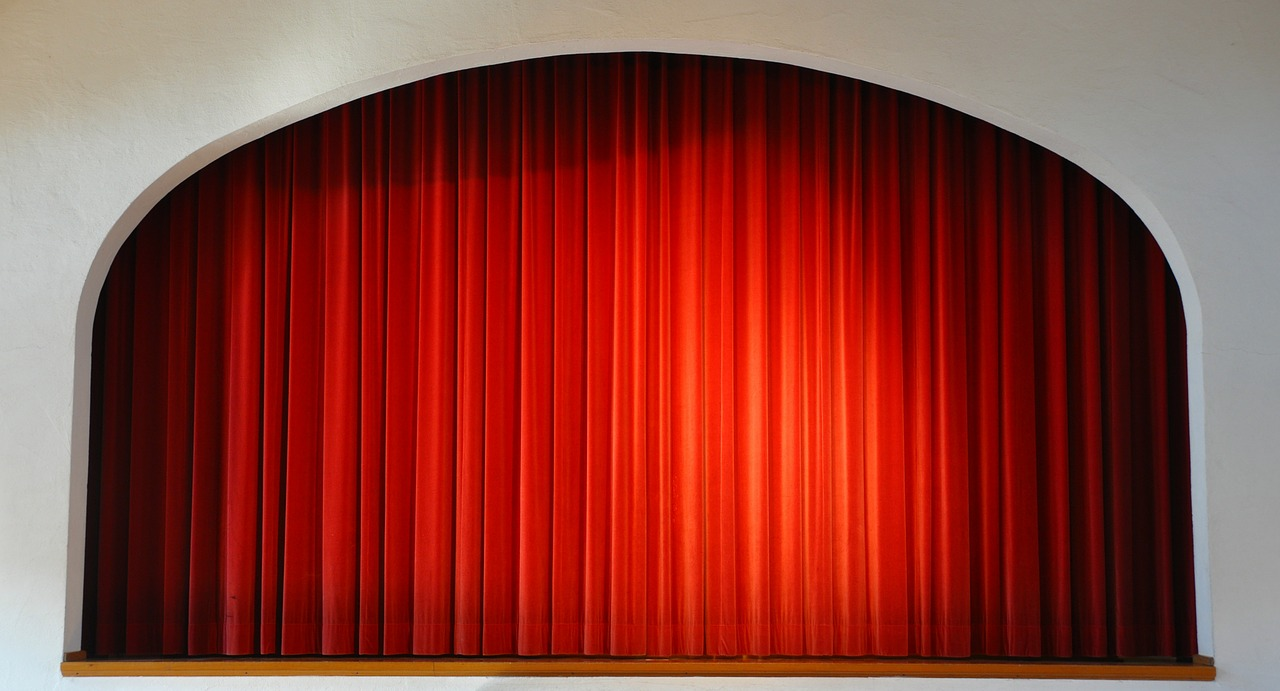
\includegraphics[width=\textwidth]{monty_hall/stage-406306_1280.jpg}}}
\only<3->{\koza[scale=.08]{0.66}}
\end{minipage}
\hfill
\begin{minipage}{.30\textwidth}
\includegraphics<1>[width=\textwidth]{monty_hall/koza.jpg}
\includegraphics<2-4>[width=\textwidth]{monty_hall/stage-406306_1280.jpg}
\includegraphics<5>[width=\textwidth]{monty_hall/curtain-152112_1280.png}
\only<3-4>{\koza[scale=.08]{0.66}}
\only<5->{\koza[scale=.08]{1}}
\end{minipage}
\end{frame}
\begin{frame}{Credits}
\begin{itemize}
\item koza: Photographer: Armin Kübelbeck, CC-BY-SA, Wikimedia Commons, \url{http://creativecommons.org/licenses/by-sa/3.0/}, \url{http://commons.wikimedia.org/wiki/File:Hausziege_04.jpg}
\item ferrari: domena publiczna \url{http://commons.wikimedia.org/wiki/File:Ferrari_California_Paris_August_2010.jpg}
\item kurtyny: domena publiczna \url{http://pixabay.com/pl/etap-kurtyna-teatr-czerwony-406306/} \url{http://pixabay.com/pl/kurtyna-etap-teatr-filmy-kino-152112/}
\end{itemize}
\note<1>
{
	Niech $S_i$ odpowiada zdarzeniu \emph{w bramce $i$ jest samochód}, a $O_i$ zdarzeniu \emph{bramka $i$ została odsłonięta}.
	Nie wiemy gdzie jest samochód, więc zakładamy jednostajne prawdopodobieństwa a priori: $P(S_i)=\frac{1}{3}$.
	Oczywiście $P(O_i|S_i)=0$.
	Załóżmy, że gracz wybiera bramkę 2, a prowadzący odsłania bramkę 3 (wybór konkretnych numerów nie ma znaczenia, problem jest symetryczny).
	Załóżmy, że prowadzący odsłania z identycznym prawdopodobieństwem, jeżeli ma wybór: $P(O_1|S_2)=P(O_3|S_2)=\frac{1}{2}$.
	Oczywiście $P(O_3|S_1)=P(O_1|S_3)=1$, bo $O_2$ jest zablokowane przez wybór gracza.
	Zatem
	\[ P(S_1|O_3)=\frac{P(O_3|S_1)P(S_1)}{P(O_3|S_1)P(S_1)+P(O_3|S_2)P(S_2)+P(O_3|S_3)P(S_3)} = \frac{1\cdot \frac{1}{3}}{1\cdot \frac{1}{3} + \frac{1}{2}\cdot \frac{1}{3} + 0} = \frac{2}{3} \]
	\[
	P(S_2|O_3)=1 - P(S_1|O_3) = \frac{1}{3}
	\]
}
\end{frame}

\end{document}

% \newlength{\koza}
% \setlength{\koza}{1357pt*\real{.8}}
% 
% \begingroup\edef\x
% {
% 	\endgroup
% 	\noexpand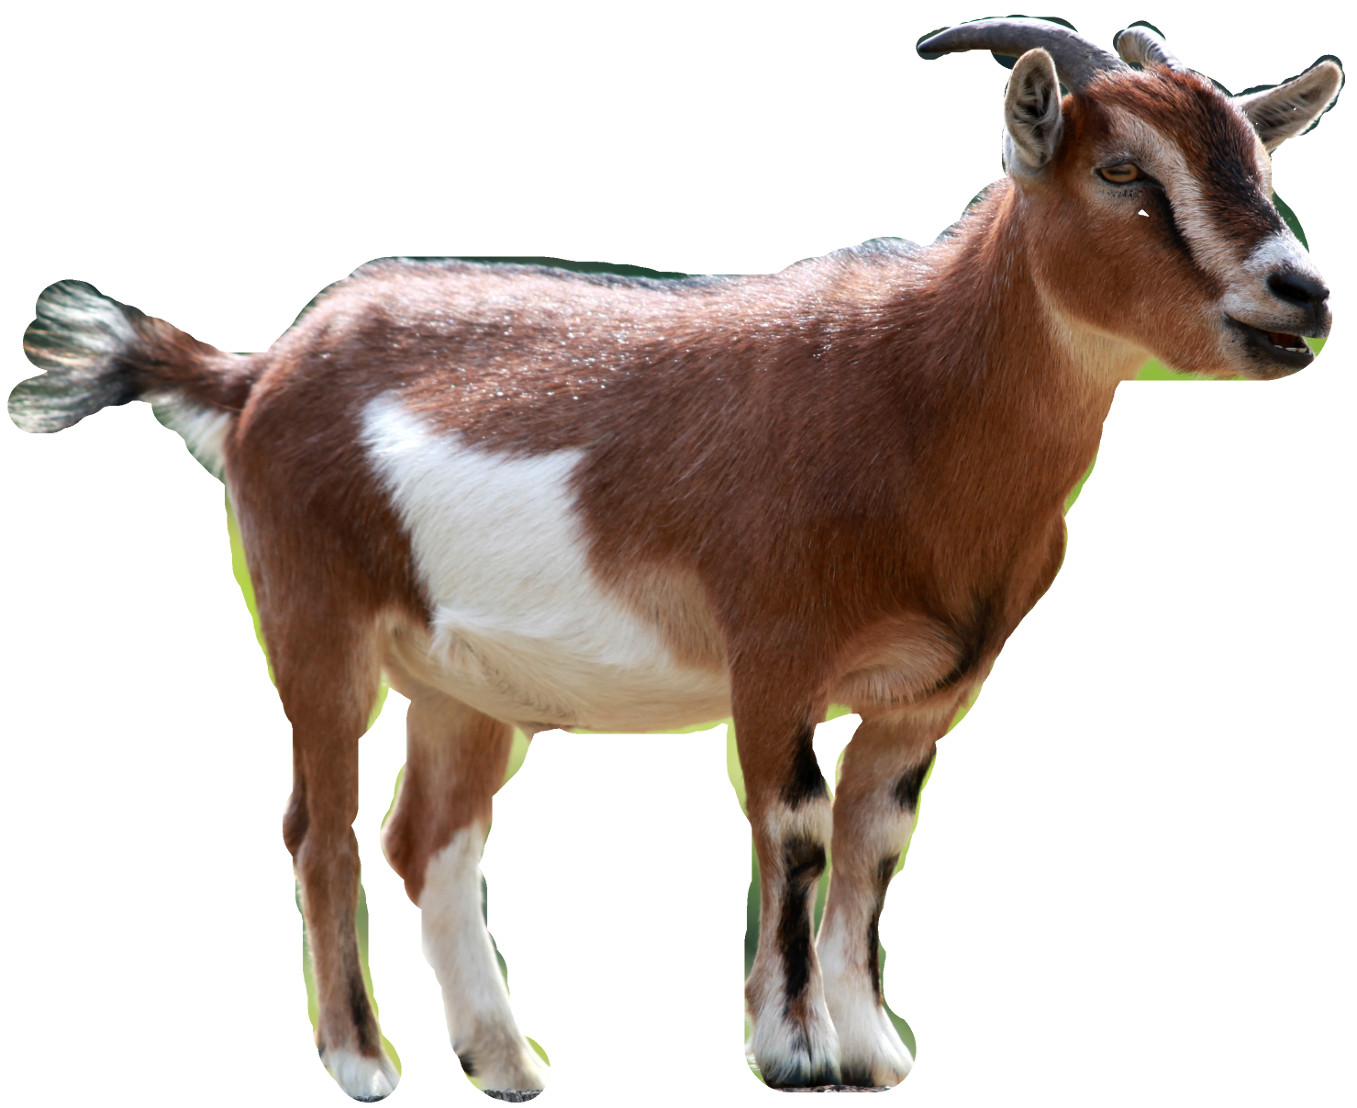
\includegraphics[clip, scale=.1, viewport=0 0 {\the\koza} 1108pt]{monty_hall/koza.jpg}
% 	%\noexpand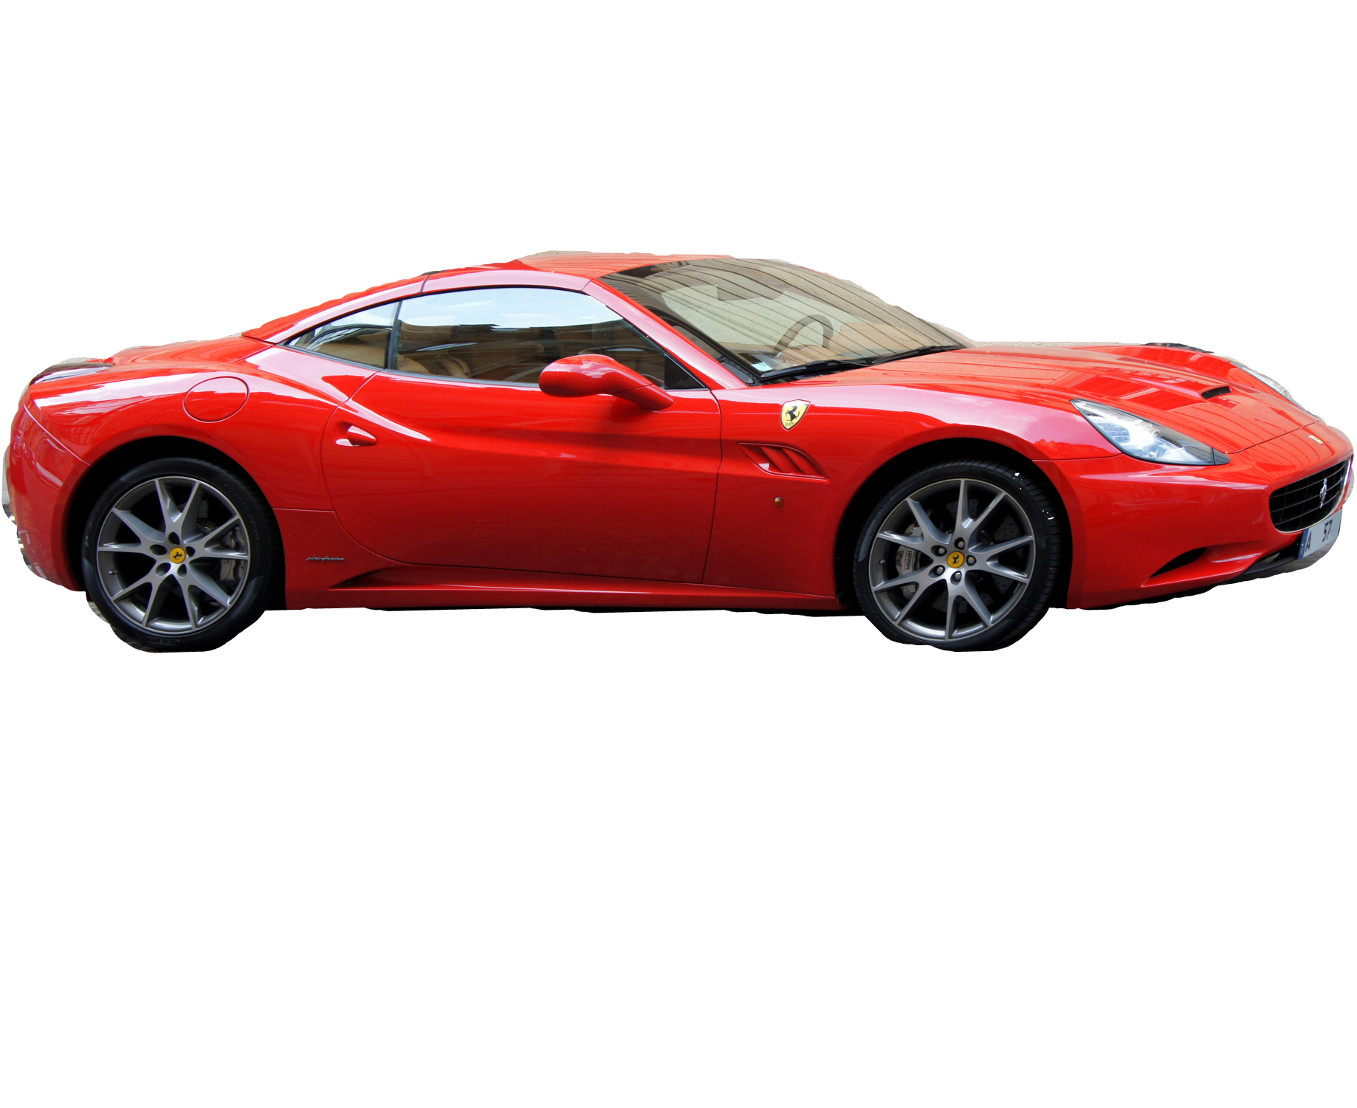
\includegraphics[clip, scale=.1, viewport={\the\ferrari} 0 3676pt 1108pt]{monty_hall/ferrari.jpg}
% 	\noexpand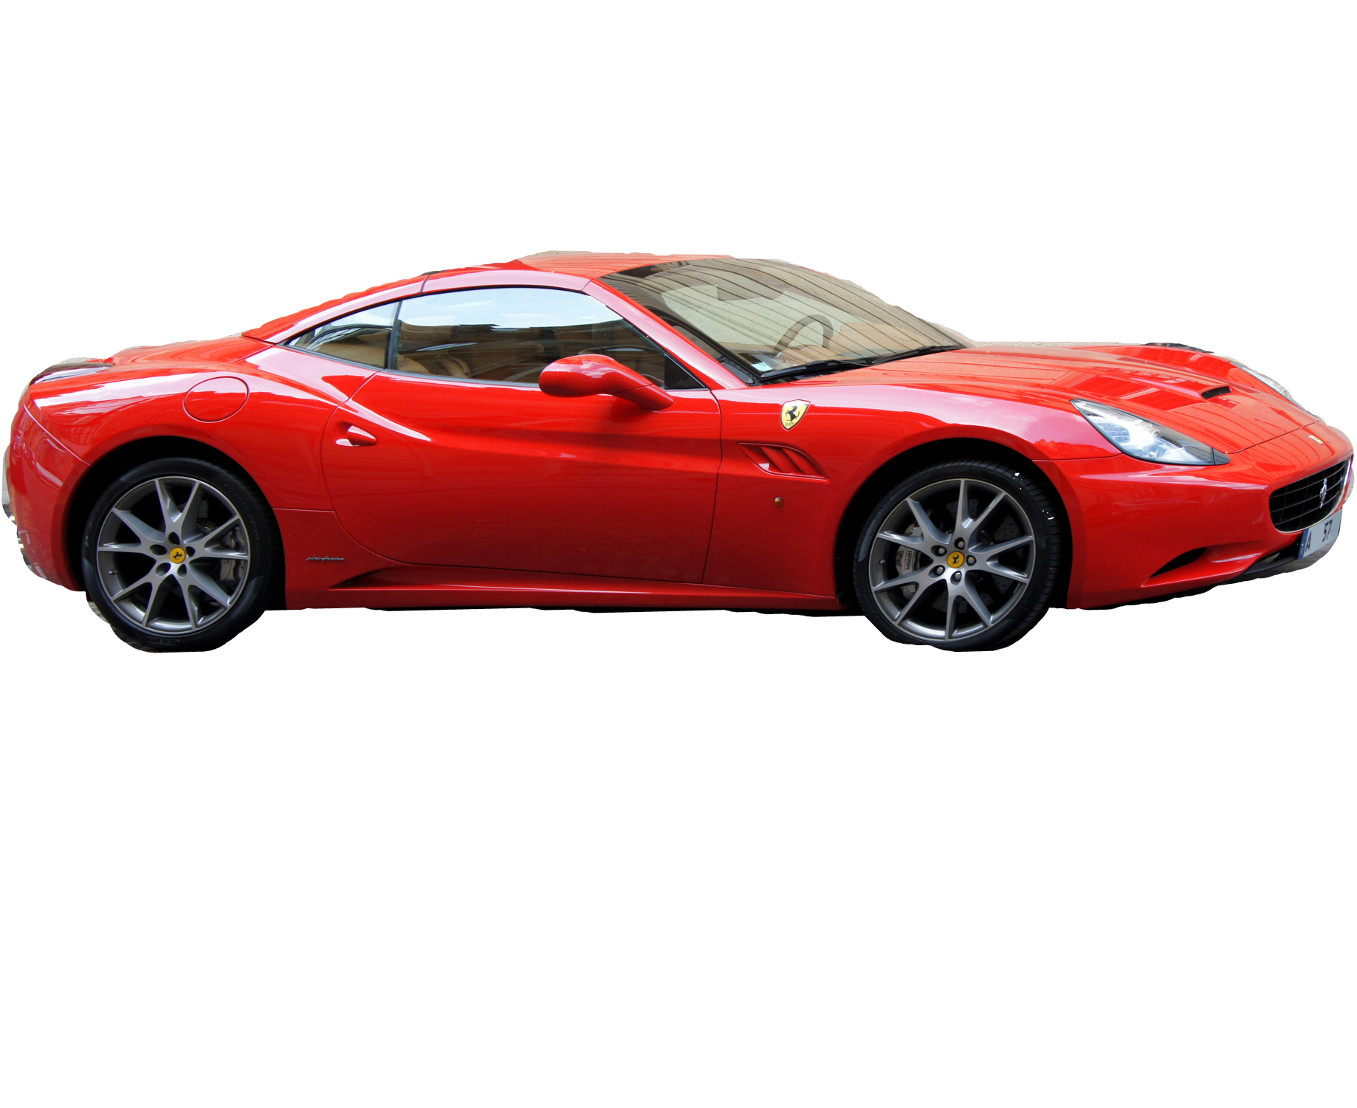
\includegraphics[clip, scale=.1, viewport={\the\koza} 0 1357pt 1108pt]{monty_hall/ferrari.jpg}
% }
% \x
%\def\x{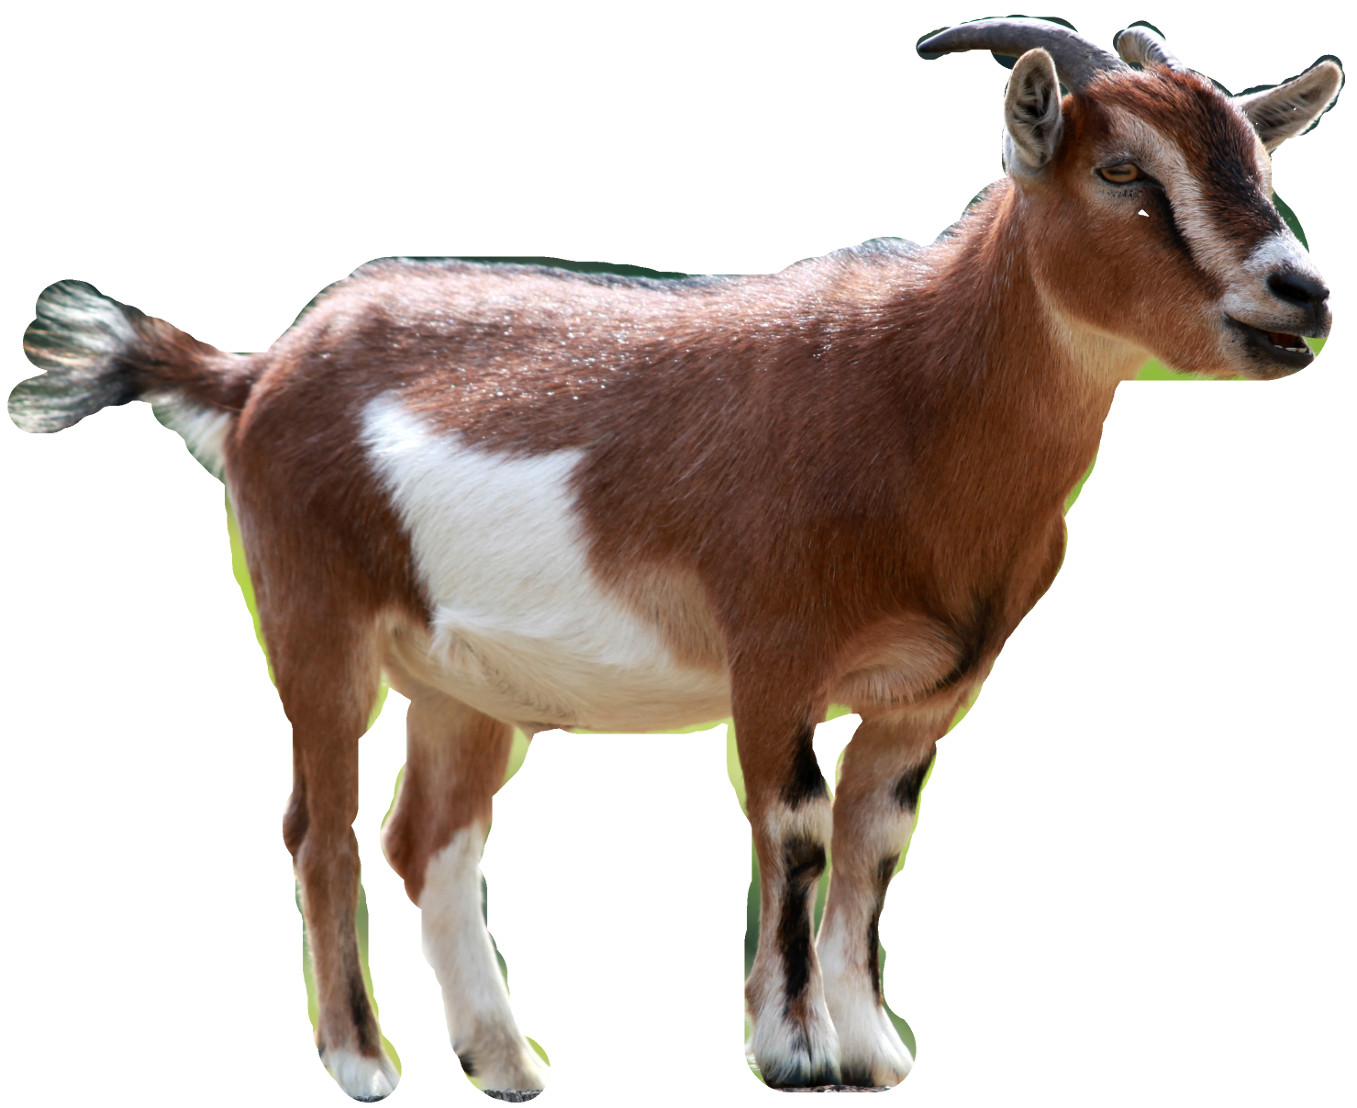
\includegraphics[scale=.1,clip,viewport=0 0 }\expandafter\x\the\koza 1108]{monty_hall/koza.jpg}}
%\setlength{\kozain}{\koza*\ratio{1}{72}}
%\begin{tikzpicture}
%\node (koza) {\x};
%%\node (ferrari) [xshift=\koza]  {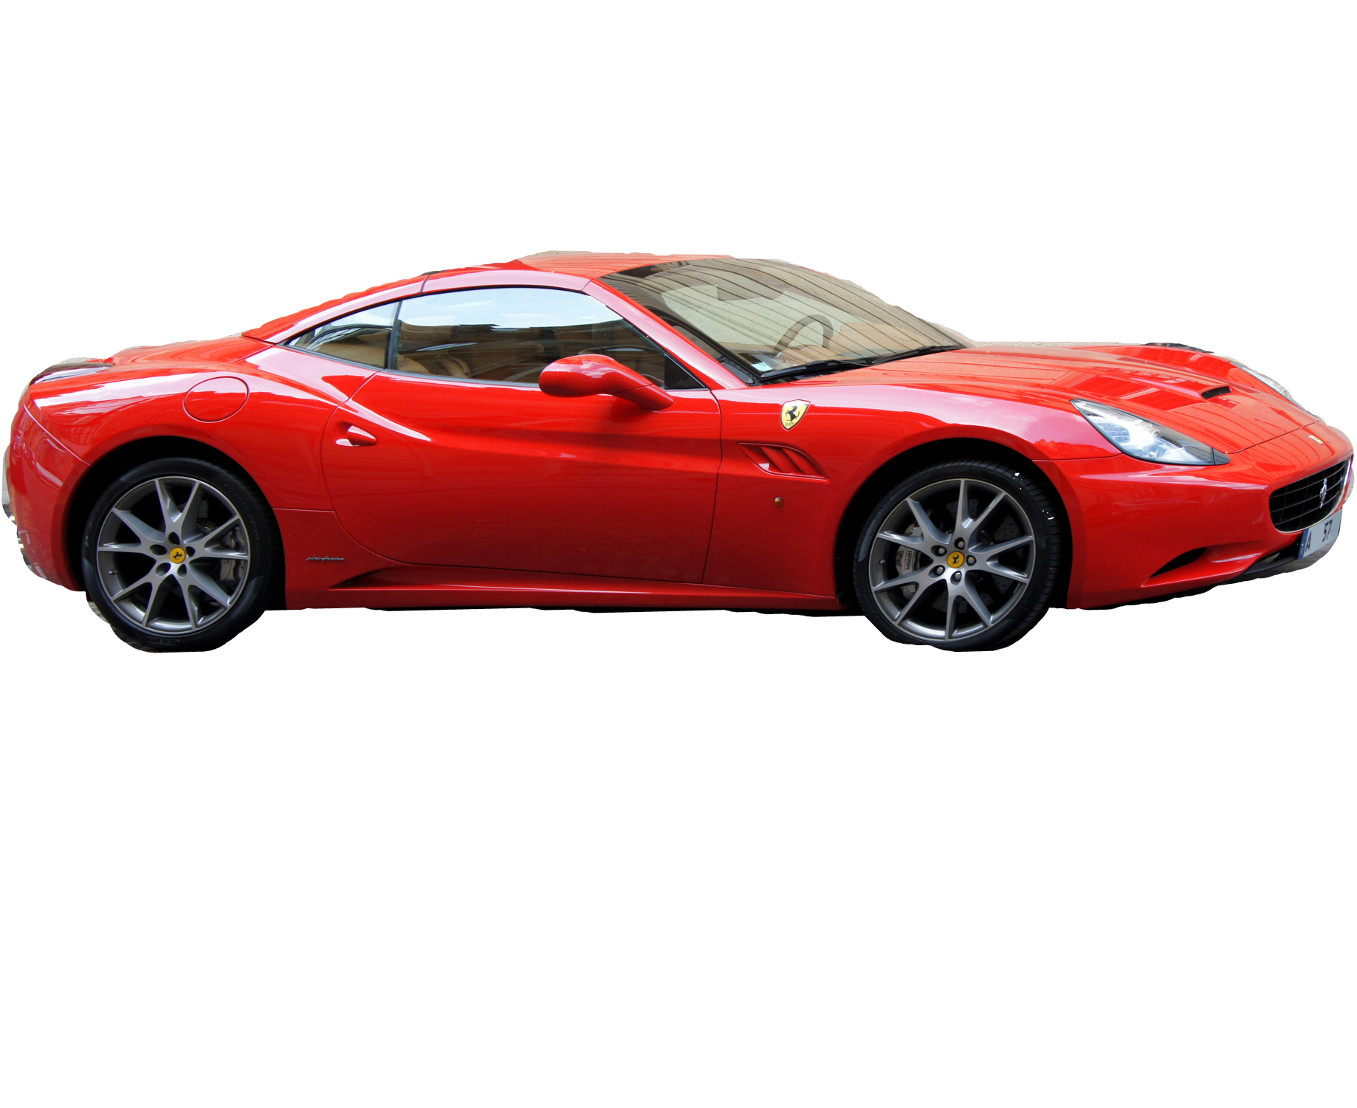
\includegraphics[scale=.1,clip,viewport=\ferrari 0 3676 1108]{monty_hall/ferrari.jpg}};
%\end{tikzpicture}

